% !TeX root = ../main.tex
\chapter{Survey and System Analysis}
\label{chap:khao-sat-phan-tich-he-thong}

\section{Survey of Current E-learning Practices and AI Needs in Modern LMS}
\label{sec:khao-sat-thuc-trang-elearning}

For many years, Learning Management Systems (LMS) have played a central role
in organizing digital classrooms. An LMS helps instructors distribute
materials, assign tasks, create quizzes, manage grades, monitor learning
progress, and communicate with learners. However, most traditional LMSs were
designed primarily around \textbf{course administration} rather than
\textbf{adaptive learning support}. Learning content is still usually created
manually, the learning experience remains mostly linear, and personalization
based on each learner's competence is still limited.

The rapid development of Generative AI opens the possibility of transforming an
LMS from a content storage and distribution system into an intelligent support
layer that can analyze documents, create micro-learning materials, generate
questions, support context-aware Q\&A, and provide learning signals for
instructors. Therefore, before designing the proposed system, this thesis
surveys current E-learning workflows, bottlenecks in learning-material
creation, and core AI needs in modern LMSs.

\subsection{Learning Organization Workflow in Traditional LMS}

A course in a traditional LMS is usually organized into courses,
modules/topics, materials, assignments, quizzes, forums, announcements, and a
gradebook. The instructor is the main designer: preparing materials, dividing
content by week or chapter, uploading files, creating assessments, configuring
deadlines, and monitoring learner results.

A common workflow can be described as follows:

\begin{enumerate}
    \item \textbf{Course initialization.} The instructor or administrator
          creates a course shell in the LMS and configures course information,
          enrollment, schedule, and access rights.
    \item \textbf{Content organization.} The instructor uploads slides, PDF
          files, additional readings, lecture videos, or external links into
          each learning module.
    \item \textbf{Learning activity design.} The instructor creates
          assignments, quizzes, discussions, or other interactive activities.
    \item \textbf{Assessment and feedback.} Learners submit work, the system
          records scores, and instructors grade, give feedback, and update the
          gradebook.
    \item \textbf{Progress monitoring.} The instructor uses basic LMS reports
          such as access count, completion rate, and average score to assess
          the class situation.
\end{enumerate}

This workflow is suitable for online classroom management, but it does not
fully solve automated course-authoring, personalized learning, or real-time
learner-support problems. Traditional LMSs store a large amount of learning
data, but often do not use it deeply to adapt content, detect knowledge gaps,
or recommend suitable learning activities.

\subsection{Current Workflow for Creating Learning Materials and Assessments}

In practice, creating digital learning materials still depends heavily on
instructor effort. Given an input such as a textbook, slide deck, academic PDF,
or lecture video, the instructor must read, summarize, select key ideas,
convert them into short lessons, write questions, prepare answers and
explanations, check errors, and then enter the result back into the LMS.

\begin{longtable}{|p{3cm}|p{3cm}|p{4cm}|p{4cm}|}
\caption{Current workflow for creating learning materials and assessments}
\label{tab:quy-trinh-tao-hoc-lieu-hien-tai}\\
\hline
\textbf{Activity} & \textbf{Common input} & \textbf{Manual operation} & \textbf{Risk / limitation} \\
\hline
\endfirsthead
\hline
\textbf{Activity} & \textbf{Common input} & \textbf{Manual operation} & \textbf{Risk / limitation} \\
\hline
\endhead
Prepare lesson content & Textbook, PDF, slides, DOCX & Read materials, select key ideas, rewrite as lessons & Time-consuming and easy to miss important content \\
\hline
Create micro-content & Chapter / lesson content & Split content, write summaries, key concepts, and flashcards & Uneven quality across lessons and dependent on instructor experience \\
\hline
Create quizzes & Learning Outcome, lesson content & Write questions, answers, distractors, and explanations & Difficult to ensure sufficient knowledge coverage and Bloom levels \\
\hline
Map content to outcomes & Course syllabus, learning outcomes & Read the syllabus and map each content item to LOs & Inconsistent and hard to update when materials change \\
\hline
Upload to LMS & Materials, quizzes, rubrics & Perform multi-step data entry in the LMS & Time-consuming and prone to formatting errors \\
\hline
Monitor results & Quiz scores, learning logs & Inspect reports manually & Hard to detect weak learners by individual competence early \\
\hline
\end{longtable}

For large classes or courses with many materials, manual work becomes a major
bottleneck. Even when instructors have strong expertise, converting knowledge
into short, interactive, frequently assessed learning units still takes
substantial time. This reduces the ability to update learning materials quickly,
especially in technology courses whose content changes rapidly.

\subsection{Limitations of Traditional LMS}

\subsubsection*{a. Heavy dependence on manual instructor operations}

Traditional LMSs provide tools to enter, manage, and distribute content, but
most of them do not understand the learning materials themselves. The system
does not automatically know which concepts a PDF contains, how many short
lessons it should be divided into, whether questions should target recognition
or application, or which part should be emphasized for weaker learners.
Therefore, instructors still perform the whole conversion from raw material to
learning activity.

This dependence increases course operation costs. With the same input material,
different instructors may create content with different levels of detail and
styles, causing inconsistent material quality across classes or semesters.

\subsubsection*{b. Limited personalization for learners}

Many LMSs organize content along a single common path for the whole class.
Learners usually study the same module order, take the same quiz set, and
receive the same type of feedback. This approach does not fully reflect
differences in background knowledge, learning speed, and personal goals.

Learning data such as quiz history, time spent on content, retake count,
frequently missed questions, and chatbot topics can provide important signals
about learner competence. Without an intelligent analysis layer, these signals
are often displayed only as static reports and are not transformed into
specific learning recommendations.

\subsubsection*{c. Lack of course-context-aware learning assistants}

In online learning, learners often struggle when studying outside class hours.
If they do not understand a concept, they may email the instructor, ask peers,
search the Internet, or use public LLMs. These approaches have limitations:
responses may be slow, information may not align with course materials, or
answers may not match the interpretation intended by the instructor.

A modern LMS needs a learning assistant that can retrieve course materials,
answer within the provided content, and cite sources clearly. This allows
learners to receive 24/7 support while maintaining consistency with official
lectures and documents.

\subsubsection*{d. Limited competence analysis and early intervention}

Traditional reports often focus on aggregate scores such as quiz scores,
assignment scores, completion rates, or access counts. These metrics are useful
but insufficient for deeper questions: which Learning Outcome a learner is weak
in, which group risks falling behind, which content causes the most confusion,
or which question has poor quality.

Without competence-level analysis, instructors have difficulty intervening at
the right time. For example, two learners with the same 6/10 quiz score may be
weak in completely different knowledge groups. An effective learning-support
system should connect assessment results with a skill map or Learning Outcomes
to produce actionable signals.

\subsection{Core AI Features in Modern LMS}

\subsubsection*{a. Content generation and Micro-learning}

Content generation is one of the most practically valuable AI applications in
an LMS. A system can receive raw materials such as PDF, DOCX, slides, or video
transcripts, extract key knowledge, and convert it into short learning units
such as lesson summaries, key concept cards, flashcards, or quiz questions.

When combined with micro-learning, AI does not merely summarize content; it
helps divide knowledge into digestible units. Each card can focus on a concept,
example, self-check question, or common misconception. This matches short,
repetitive, mobile-friendly learning habits.

However, in education, AI-generated content should not be published directly.
The system needs instructor review, source traceability, and editability before
learners access the content.

\subsubsection*{b. Personalized learning paths}

Adaptive Learning adjusts content, difficulty, and learning activities based on
each learner's actual competence. AI can analyze learning history, quiz
results, interaction time, Learning Outcome mastery, and learner questions to
recommend the next module.

For example, if a learner frequently misses ``application'' questions in a
topic, the system can recommend revisiting key concept cards, practicing
flashcards, or taking an easier exercise set before returning to the main
quiz. In this approach, the LMS is no longer a static content list but a
learning environment that responds to individual progress.

Within this thesis, Adaptive Learning is positioned at a curriculum-aware
level: the system links micro-content and quizzes to Learning Outcomes, making
it possible to monitor mastery and recommend suitable review content.

\subsubsection*{c. Virtual tutor and learning assistant}

An AI Tutor or learning chatbot can act as an assistant that answers questions
according to course context. The difference between an educational chatbot and
a general chatbot lies in its ability to stay aligned with official materials,
cite sources, and limit answers to the course scope.

In modern architecture, this function is usually built with
Retrieval-Augmented Generation (RAG). When a learner asks a question, the
system finds relevant passages in the course knowledge base, passes them into
the LLM prompt, and asks the model to answer based on those sources. This helps
reduce hallucination, increase verifiability, and better fit educational
contexts.

\subsubsection*{d. Learning analytics and Skill Mapping}

AI can help summarize learning data into competence maps. Instead of displaying
only final scores, the system can analyze quiz results by Learning Outcome,
topic group, Bloom level, or skill. This helps instructors know where the class
is weak and which learners need early support.

Skill Mapping is especially useful when a course has explicit outcomes. Each
quiz question can be linked to one or more Learning Outcomes; each correct or
incorrect answer updates the corresponding mastery level. The system can then
display learning analytics by competence rather than aggregate score only.

\subsubsection*{e. Intelligent exam monitoring}

AI Proctoring uses computer vision, face recognition, behavior analysis, and
anomaly detection to support online exam monitoring. This feature group is
often mentioned in modern LMSs, especially for remote assessment.

However, AI Proctoring raises privacy, accuracy, model bias, and learner
experience issues. Therefore, in this thesis, AI Proctoring is considered a
market reference capability rather than a core implemented feature. The
proposed system focuses on learning-material generation, quizzes, RAG tutor,
review workflow, curriculum-aware learning, and LMS integration.

\subsection{Limitations of Using LLMs Directly in Education}

\subsubsection*{a. Hallucination}

LLMs can generate natural text but cannot guarantee that every answer is
correct. In education, a wrong answer written confidently can seriously mislead
learners. This risk is especially important when AI explains technical
knowledge or creates assessment questions.

Therefore, directly using an LLM as a free-form ``ask anything, answer
anything'' service is unsuitable for LMS use. The system must reduce risk by
retrieving source materials, requiring citations, limiting answer scope, using
structured output, and routing generated content through instructor review.

\subsubsection*{b. Poor alignment with course materials}

A general LLM can answer based on broad training knowledge, but the answer may
not match the materials, learning outcomes, or explanation style of a specific
course. Two courses on the same topic may have different scopes, terms, and
expected levels.

Therefore, the system must treat course materials as the primary source of
truth. With a retrieval-first architecture, AI answers or generates content
based on passages that have been processed, chunked, embedded, and stored in
the course retrieval repository.

\subsubsection*{c. Lack of pedagogical control}

An LLM can quickly generate questions or summaries, but it does not
automatically guarantee alignment with learning objectives, Bloom level,
difficulty, learning duration, or the instructor's pedagogical strategy.
Without constraints, generated content may be too easy, too difficult,
duplicated, or off-topic.

An educational AI system needs pedagogical metadata: Learning Outcome, Bloom
level, question type, source material, difficulty, review status, and content
version. These metadata make generated content reviewable, editable,
publishable, and evaluable.

\subsubsection*{d. Lack of LMS and learning-data integration}

When instructors or learners use LLMs outside the LMS, generated data is often
fragmented: prompts in one place, learning content in another, quizzes
elsewhere, and scores still entered manually into the LMS. This breaks the
continuity of the learning workflow.

An AI system should integrate with the LMS to receive user identity, course
context, roles, roster, gradebook, and learning-activity links. AI then becomes
an extension layer in the teaching and learning process rather than a separate
text-generation tool.

\subsection{Research Problem Synthesis}

The analysis above shows that the research problem is not merely ``using AI to
generate quizzes'', but designing a controlled, contextual, and extensible AI
system for LMS support. The system must address the following requirements
simultaneously:

\begin{itemize}
    \item Automatically process multi-format academic documents and lecture
          videos.
    \item Convert raw materials into structured micro-content, flashcards, and
          quizzes.
    \item Link generated content with Learning Outcomes and pedagogical
          metadata.
    \item Provide an RAG-based AI Tutor Chatbot that answers according to
          course materials.
    \item Allow instructors to review, edit, and publish content before
          learners can access it.
    \item Integrate with Canvas LMS through LTI 1.3 to use identity, course
          context, and gradebook.
    \item Satisfy requirements for security, cost control, logging, monitoring,
          and AI quality evaluation.
\end{itemize}

Therefore, the proposed system is designed as an \textbf{AI Extension Layer for
LMS}: it does not replace the whole LMS, but adds an AI processing layer for
document-to-micro-content, quiz generation, RAG tutoring, curriculum-aware
learning, and human-in-the-loop review.

\section{Survey of AI Systems and Solutions in Education}
\label{sec:khao-sat-giai-phap-ai-giao-duc}

Current AI solutions in education can be grouped into three main categories:
commercial LMSs with built-in AI, learning platforms or EdTech tools using
Generative AI, and open-source LMSs that can be extended through plugins or
integration standards. Each group has strengths and limitations when compared
with the problem targeted by this thesis.

\subsection{Commercial LMSs with Built-in AI}

\subsubsection*{a. Canvas LMS / Instructure IgniteAI}

Canvas LMS is one of the popular LMS platforms in higher education.
Instructure's AI capabilities are positioned under IgniteAI, including support
for course-content search, quiz-question generation, discussion summarization,
translation, rubric generation, grading support, and administrative agent tasks
in newer product packages \cite{instructure-ai}.

Canvas is strong because it provides a complete LMS ecosystem: course
management, assignments, quizzes, gradebook, roles, APIs, and LTI support. For
this thesis, Canvas is suitable as the base LMS, while the proposed AI system
operates as an external tool integrated through LTI 1.3.

However, Canvas commercial AI capabilities depend on Instructure's service
packages and deployment environment. For a research objective that needs AI
architecture autonomy, building a separate AI Extension Layer provides more
control over document processing, model selection, RAG design, data control,
and review-interface customization.

\subsubsection*{b. Blackboard Learn AI Design Assistant}

Blackboard Learn provides AI Design Assistant to help instructors build course
structures, create modules, suggest content, and support assessment, rubric,
and image creation based on course context \cite{blackboard-ai}. This is a
representative example of bringing Generative AI into LMS authoring workflows.

Its strength is that AI is embedded directly into the instructor experience,
reducing the effort required to draft a course. However, the feature remains
inside a closed commercial ecosystem and is difficult to customize deeply for a
research pipeline such as document parsing, vector search, curriculum graph, or
review state machine.

\subsubsection*{c. Docebo}

Docebo is an LMS/Learning Platform oriented toward enterprise training, with a
strong focus on learning-administration automation, content tagging, skill
mapping, content search, and AI-assisted administration \cite{docebo-ai}.
Docebo suits organizations that need large-scale training, learner grouping by
job role, and skill management in business contexts.

Docebo's value lies in content intelligence and skill-based learning. However,
for this thesis, Docebo is not the optimal base because the system must focus
on academic-course environments, course materials, micro-content, quizzes by
Learning Outcome, and self-hosted or deeply Canvas-integrated deployment.

\subsubsection*{d. TalentLMS}

TalentLMS emphasizes simplicity in course creation and internal training.
AI features such as TalentCraft, course-description generation, image
generation, content generation, and question generation from prompts or
existing content help instructors/trainers shorten course design time
\cite{talentlms-ai}.

TalentLMS is easy to approach and suitable for corporate training or short
courses. However, from the research requirements of this thesis, it is not an
open platform for implementing customized AI pipelines such as
document-grounded RAG, dedicated vector databases, curriculum graphs, and Canvas
gradebook integration through LTI.

\subsubsection*{e. CYPHER Learning AI 360}

CYPHER Learning develops AI 360 / CYPHER Agent to support course creation,
learning-content creation, assessment, rubrics, and personalized learning
\cite{cypher-ai}. The platform reflects the ``AI-first'' LMS trend, where AI
participates from course design to learner-experience operation.

CYPHER is strong in authoring automation. Similar to other commercial LMSs,
however, it is bounded by vendor architecture and customization options. For a
thesis that must demonstrate technical design, building an AI Extension Layer
makes the architectural decisions clearer: chunking, embedding, RAG,
asynchronous pipelines, human review, and observability.

\subsection{Learning Platforms and EdTech Tools Using Generative AI}

\subsubsection*{a. Coursera AI-assisted Course Builder}

Coursera provides Course Builder as an AI-assisted authoring tool that helps
instructors create customized courses and receive relevant content suggestions
from the Coursera ecosystem \cite{coursera-builder}. This approach leverages a
large existing content repository to support faster course creation.

However, Coursera is a learning/MOOC platform rather than an internally
deployed LMS based on open integration standards. It is suitable for course
distribution on Coursera, but it does not directly solve integration with
Canvas, processing instructor-owned materials, or publishing quiz results into
an institution's LMS gradebook.

\subsubsection*{b. Quizlet AI Study Tools}

Quizlet focuses on personal study tools such as flashcards, practice tests,
study guides, PDF summarizers, and flashcard creation from notes, slides, or
documents \cite{quizlet-ai}. It is a representative example of using AI to
convert documents into concise review materials.

Quizlet is strong in fast, focused, personal learning experiences. However, it
is not a full LMS: it does not manage the complete course lifecycle, replace an
official gradebook, support formal instructor/learner review workflows, or
align tightly with the Learning Outcomes of a specific course.

\subsubsection*{c. Khanmigo}

Khanmigo is Khan Academy's AI assistant, positioned as a personal tutor for
learners and a teaching assistant for teachers \cite{khanmigo}. Its approach is
notable because it does not simply provide direct answers; it guides, prompts,
and helps learners reason.

Khanmigo demonstrates the strong potential of AI Tutors in education. However,
it mainly operates within Khan Academy's content ecosystem. In this thesis, an
important requirement is that the chatbot must retrieve each LMS course's own
materials and connect with instructor-provided micro-content, quizzes, and
Learning Outcomes.

\subsubsection*{d. Tools for generating quizzes / flashcards from documents}

In addition to major platforms, the market has many specialized tools that
allow users to upload PDFs, slides, or notes to automatically create
flashcards, quizzes, summaries, or study guides. These tools are useful for
personal study and reduce review-material preparation time.

However, standalone tools usually have several limitations:

\begin{itemize}
    \item They do not integrate deeply with LMSs, rosters, gradebooks, and
          access control.
    \item They do not ensure that learning data is managed according to an
          institution's policy.
    \item They lack formal instructor review workflows.
    \item They lack links with Learning Outcomes, Bloom Taxonomy, and learning
          analytics.
    \item They make it difficult to control source materials, content versions,
          and question quality.
\end{itemize}

Thus, they are useful local support tools, but they are not sufficient as the
architectural foundation for a controlled LMS system that automatically creates
micro-content and quizzes.

\subsection{Open-source LMSs and AI Extensibility}

\subsubsection*{a. Moodle and AI Subsystem / AI Plugins}

Moodle is a popular open-source LMS with a large plugin community and an AI
direction through its AI Subsystem. Moodle describes the AI Subsystem as a
foundation for integrating AI tools into the LMS without locking into one
provider \cite{moodle-ai}.

Moodle's strengths are openness, community, and customizability. However, the
plugin model can also lead to fragmented experiences if AI features are added
separately. For this thesis, Moodle is a feasible AI integration option, but
the system prioritizes Canvas because it needs to exploit LTI 1.3, APIs,
gradebook, and the project's concrete deployment context.

\subsubsection*{b. Canvas LMS Open Source}

Canvas LMS has an open-source codebase maintained on GitHub by Instructure
\cite{canvas-oss}. This allows LMS architecture study, self-deployment, and
external-service integration. Canvas also provides APIs and LTI support, which
fits the external-tool approach.

Nevertheless, modifying Canvas core directly to add AI would create high
maintenance costs, especially when LMS versions need to be upgraded. Therefore,
a better approach is to build the AI system as an independent service,
integrated through LTI and APIs, with minimal intervention in the LMS core.

\subsubsection*{c. Open edX}

Open edX is a powerful open-source platform for MOOCs and large-scale online
learning. It supports learning-experience extensions through XBlock and LTI
1.3 / LTI Advantage integration \cite{openedx-lti}. Open edX suits
organizations that need to deliver online courses at scale with complex content
structures and interactive components.

However, Open edX has high deployment and operation complexity. If the main
goal is to build an AI Extension Layer for document processing, micro-content
generation, quizzes, and chatbots, starting with Canvas/LTI keeps the system
scope clearer and more focused on AI.

\subsubsection*{d. Sakai}

Sakai is a long-standing open-source LMS used in higher education and supports
the LTI standard \cite{sakai-lms}. Its strengths are community orientation,
extensibility, and academic use cases.

Compared with Moodle, Canvas, or Open edX, the popular AI ecosystem around
Sakai is less prominent. AI integration usually requires custom tools or
external services. Therefore, Sakai is considered a reference platform for LMS
extensibility comparison, but not the main choice in this thesis.

\subsection{Comparison of Solution Groups}

\begingroup
\footnotesize
\setlength{\tabcolsep}{3pt}
\begin{longtable}{|p{2.4cm}|p{2.9cm}|p{3cm}|p{2.8cm}|p{3cm}|}
\caption{Comparison of AI solution groups in education}
\label{tab:so-sanh-giai-phap-ai-giao-duc}\\
\hline
\textbf{Criterion} & \textbf{Commercial LMS with AI} & \textbf{EdTech / AI learning tools} & \textbf{Open-source LMS} & \textbf{Proposed system} \\
\hline
\endfirsthead
\hline
\textbf{Criterion} & \textbf{Commercial LMS with AI} & \textbf{EdTech / AI learning tools} & \textbf{Open-source LMS} & \textbf{Proposed system} \\
\hline
\endhead
Learning-material generation & Available and increasingly strong in authoring & Strong in flashcards, quizzes, summaries & Depends on plugins / custom work & Main focus: document/video to micro-content \\
\hline
LMS integration & Very strong inside the vendor ecosystem & Usually weak or indirect & Can integrate through plugins/LTI & Canvas integration through LTI 1.3 \\
\hline
Personalized learning & Available in some platforms & Mostly personal-study personalization & Depends on implementation & Curriculum-aware, based on LOs and learning results \\
\hline
Retrieval over course materials & Available but platform-dependent & Inconsistent & Depends on integrated pipeline & RAG over each course's materials \\
\hline
Instructor review & Available at authoring level & Usually not an LMS workflow & Depends on plugins & Human-in-the-loop review before publish \\
\hline
Data and model control & Limited by vendor dependency & Limited & Higher if self-hosted & Custom services, vector DB, and storage \\
\hline
Observability and cost control & Vendor-dependent & Usually limited & Must be built & Explicit logging, metrics, and cost tracking \\
\hline
Fit for this thesis & Useful reference & Useful reference for learning UX & Useful reference for extensibility & Best fit for the research objective \\
\hline
\end{longtable}
\endgroup

The comparison shows that no existing group fully satisfies the thesis
requirements. Commercial LMSs are strong in administration and internal
integration but difficult to customize deeply. EdTech tools are strong in
learning experience and quick material generation but are not complete LMSs.
Open-source LMSs are flexible but require substantial integration work and may
lead to fragmented plugins.

\subsection{Technology Gap Analysis}

\subsubsection*{a. Traditional LMSs are strong in administration but AI remains fragmented}

LMSs are well designed for course administration, but when AI is added, many
systems introduce isolated features such as search, rubric generation, quiz
assistants, or summaries. This improves part of the workflow but does not
necessarily form a unified pipeline from input materials to micro-content,
quizzes, review, publish, and analytics.

\subsubsection*{b. AI learning tools are strong in generation but are not full LMSs}

Tools such as Quizlet or flashcard generators can create learning content
quickly, but they lack LMS functions such as course management, roles,
enrollment, gradebook, LTI standards, learning analytics, and access control.
When used separately, learning data is detached from the institution's official
system.

\subsubsection*{c. Plugin-based solutions can fragment the experience}

Plugins are a quick extension mechanism, but they can produce inconsistent
experiences if each AI function has its own interface, data, and workflow. For
example, a quiz plugin, chatbot plugin, and analytics plugin may not share the
same document source, Learning Outcome metadata, or review mechanism.

The proposed system avoids this by designing a unified AI pipeline in which
document processing, chunking, embedding, generation, RAG, review, and
analytics share the same core data.

\subsubsection*{d. Lack of systems designed around Micro-learning, RAG, review, and LMS integration}

The most important gap is the lack of a system designed from the beginning for
the workflow: \textbf{academic document / lecture video $\rightarrow$
micro-content $\rightarrow$ quiz $\rightarrow$ review $\rightarrow$ publish
$\rightarrow$ learning and assessment in LMS}.

Such a system must combine several technical layers:

\begin{itemize}
    \item Document Intelligence for PDF, DOCX, PPTX, and video transcripts.
    \item Chunking and embedding as a semantic retrieval foundation.
    \item RAG so chatbot and generation stay grounded in course materials.
    \item Structured output for quiz, flashcard, and metadata persistence.
    \item Curriculum mapping to connect content with Learning Outcomes.
    \item Human-in-the-loop review so instructors control content before
          publishing.
    \item LTI 1.3 / Advantage to integrate with LMSs without replacing them.
    \item Observability to monitor jobs, errors, AI cost, and output quality.
\end{itemize}

This is the space targeted by the proposed system.

\subsection{Approach Analysis for the Proposed System}

\subsubsection*{a. Building a complete LMS from scratch}

The first approach is to build a new LMS from the ground up, including user
management, courses, content, quizzes, gradebook, discussions, notifications,
and analytics. Its advantage is full control over product design and data
architecture.

However, the disadvantage is a much larger development scope. Building a
complete LMS requires many foundational features that are not directly related
to the main contribution of the thesis. If too much effort is spent on the LMS
core, fewer resources remain for RAG, micro-content generation, quiz
generation, curriculum mapping, and AI safety.

\subsubsection*{b. Integrating AI into an open-source LMS}

The second approach is to choose an open-source LMS such as Moodle, Canvas Open
Source, or Open edX, then develop plugins or modify the core to add AI. This
reuses an existing LMS and allows deeper customization than closed commercial
platforms.

However, modifying LMS core increases maintenance cost and complicates version
upgrades. If many separate plugins are developed, the user experience may be
fragmented. In addition, each LMS has a different plugin architecture, so
migrating to another platform requires substantial work.

\subsubsection*{c. Building an AI Extension Layer for LMS}

The selected approach is to build an independent AI layer that integrates with
the LMS through LTI 1.3 / LTI Advantage \cite{lti-advantage}. In this model,
Canvas LMS still handles core LMS functions such as courses, users, roles,
assignments, and gradebook. The proposed system handles AI functions:

\begin{itemize}
    \item Upload and process documents / videos.
    \item Generate micro-content, flashcards, and quizzes.
    \item Store embeddings and perform semantic retrieval.
    \item Provide an RAG-based AI Tutor Chatbot.
    \item Manage content review and publishing.
    \item Track processing progress with asynchronous jobs and streaming
          updates.
    \item Record learning results and synchronize quiz scores to the LMS when
          needed.
\end{itemize}

This approach has several advantages:

\begin{itemize}
    \item \textbf{Reduced LMS-core scope.} The system does not reimplement the
          complete LMS feature set.
    \item \textbf{Better integration potential.} LTI is a common standard
          between LMSs and external tools, enabling future expansion to other
          LMSs.
    \item \textbf{Clear responsibility separation.} The LMS manages the class;
          the AI Extension Layer handles AI pipelines and micro-learning
          experiences.
    \item \textbf{Better AI data control.} Documents, chunks, embeddings,
          generated results, and review states are managed in the AI system.
    \item \textbf{Fit with the research direction.} The thesis can focus on
          document processing, RAG, structured generation, review workflow,
          security, and observability.
\end{itemize}

\subsubsection*{d. Rationale for the selected approach}

Based on the survey, the proposed system selects the \textbf{AI Extension Layer
for Canvas LMS} model. This balances practicality and research value: it reuses
an existing LMS while allowing a specialized AI pipeline to be designed
independently.

With this approach, the main contribution is not creating another LMS, but
building an AI layer capable of:

\begin{itemize}
    \item transforming academic documents and lecture videos into structured
          micro-content;
    \item generating quizzes with explanations, metadata, and Learning Outcome
          links;
    \item providing a chatbot that retrieves from course materials;
    \item supporting instructor review before publishing;
    \item integrating with Canvas through LTI 1.3;
    \item satisfying security, cost-control, and observability requirements.
\end{itemize}

Thus, the proposed system addresses the gap between two existing solution
groups: LMSs that are strong in administration but whose AI remains fragmented,
and AI learning tools that are strong in generation but lack official LMS
integration.

\section{System Actor Analysis}
\label{sec:phan-tich-tac-nhan-he-thong}

The proposed system acts as an \textbf{AI Extension Layer} connected to Canvas
LMS through LTI 1.3 / OIDC, so the actors include both human users and external
systems. Table~\ref{tab:tac-nhan-he-thong} summarizes the five main actors.

\begin{longtable}{|p{1.5cm}|p{4cm}|p{2cm}|p{6cm}|}
\caption{Main system actors}
\label{tab:tac-nhan-he-thong}\\
\hline
\textbf{Code} & \textbf{Actor} & \textbf{Type} & \textbf{Role in the system} \\
\hline
\endfirsthead
\hline
\textbf{Code} & \textbf{Actor} & \textbf{Type} & \textbf{Role in the system} \\
\hline
\endhead
AC-01 & Instructor & Human & Provides documents/videos, reviews, and publishes micro-content \& quizzes \\
\hline
AC-02 & Learner & Human & Consumes micro-content, takes quizzes, asks the chatbot, and tracks progress \\
\hline
AC-03 & Canvas LMS & System & Provides identity, course context, and gradebook through LTI 1.3 / OIDC \\
\hline
AC-04 & LLM Provider (Gemini, OpenAI) & System & Generates embeddings, micro-content, quizzes, and chatbot answers \\
\hline
AC-05 & System Administrator & Human & Operates quotas, cost, observability, and LTI Tool registration \\
\hline
\end{longtable}

\subsection{Instructor}

\textbf{Role.} The instructor creates and reviews learning content. In the
thesis's \textit{Human-in-the-loop Review} philosophy, the instructor is the
final checkpoint that ensures content quality before learners access it. AI
creates drafts, while the instructor approves and holds academic responsibility.

\textbf{Access channel.} Instructors do not log directly into the AI system.
They work inside Canvas LMS and click the registered External Tool in the
course. Canvas initiates an LTI launch and redirects to the thesis AI
interface, carrying instructor identity and course context. Protocol details
are presented in the system design chapter.

\textbf{Main responsibilities.}

\begin{itemize}
    \item Upload learning materials or course syllabi to the system.
    \item Upload / embed lecture videos so the system can generate
          timestamp-based micro-content.
    \item Monitor the AI processing progress.
    \item Review and edit generated micro-content / quizzes; add manual
          questions if needed.
    \item Publish the course, fully or by section, only after review.
    \item View the class dashboard: completion rate, average quiz score, and
          Learning Outcomes in which learners are weak.
\end{itemize}

\textbf{Technical familiarity.} Medium: able to upload files, use drag and
drop, and edit text; no deep AI knowledge is required.

\subsection{Learner}

\textbf{Role.} Learners consume micro-learning content and are the target of
personalized support.

\textbf{Access channel.} Similar to instructors, learners access the system
through Canvas without a separate login. Canvas authenticates the learner and
redirects to the AI interface with identity and the \texttt{Learner} role in
the course.

\textbf{Main responsibilities.}

\begin{itemize}
    \item Read Lesson Summaries and Key Concept Cards, and flip Flashcards in
          the suggested order.
    \item Watch lecture videos with timestamped micro-content annotations.
    \item Take quizzes and receive immediate feedback and explanations.
    \item Interact with the AI Tutor Chatbot by asking course-scoped questions
          and receiving cited answers.
    \item View personal learning progress, mastered LOs, and LOs that need
          review.
\end{itemize}

\textbf{Technical familiarity.} Basic web/app usage; no advanced technical
knowledge is required.

\subsection{LMS / External System}

\textbf{Role.} The external system provides \textbf{identity, course context,
and gradebook} for the AI system through LTI 1.3. Within this thesis, the main
LMS is \textbf{Canvas LMS}; because the design follows LTI, the same
communication model can technically be moved to other LTI 1.3-enabled LMSs
such as Moodle 4.x, Open edX, or Sakai if needed.

\textbf{Interaction responsibilities.}

\begin{itemize}
    \item \textbf{Authentication and authorization.} Canvas authenticates users
          and passes identity and roles to the AI system. The AI system does
          not manage passwords or accounts.
    \item \textbf{Course context.} Canvas sends course ID, course name, and
          course code so the AI system knows which course a document or quiz
          belongs to.
    \item \textbf{Deep Linking.} Canvas allows instructors to select specific
          documents or quizzes from the AI system and embed them into the
          course.
    \item \textbf{Grade synchronization.} The AI system pushes quiz scores to
          the Canvas gradebook through standard LTI services.
    \item \textbf{Roster synchronization} (optional). The AI system can fetch
          the course roster to support analytics.
\end{itemize}

\textbf{Characteristics.} This is a system actor, not a human actor. It is the
identity data source and score destination. The AI system acts as an
\textit{LTI Tool} with Canvas and as a \textit{client} when calling Canvas
services. Protocol details are presented in the integration design chapter.

\subsection{LLM Provider}

\textbf{Role.} The external AI service provides content-generation and
semantic-representation capabilities. In the proposed system, this component
prioritizes the \textbf{Google Gemini API}; the design allows replacement with
other providers such as OpenAI, Anthropic Claude, or self-hosted models without
changing business logic. The rationale and architectural details are presented
in the theoretical foundation and design chapters.

\textbf{Interaction responsibilities.}

\begin{itemize}
    \item Generate Micro-content: Lesson Summary, Key Concept Card, Flashcard.
    \item Generate structured quizzes classified by Bloom Taxonomy.
    \item Generate semantic representations for search.
    \item Answer AI Tutor Chatbot questions.
    \item Return usage-cost information so the system can control budget.
\end{itemize}

\textbf{Characteristics.} This is an external system actor, billed by usage and
\textbf{non-deterministic}: the same input may produce different outputs.
Therefore, the system needs cost control, fallback, and rate limiting.

\subsection{System Administrator}

\textbf{Role.} The system administrator operates the AI system side and is not
the LMS role. LMS admins are managed separately by the LMS.

\textbf{Access channel.} The administrator logs directly into a dedicated AI
system admin interface, not through Canvas.

\textbf{Main responsibilities.}

\begin{itemize}
    \item Register the AI system as an LTI Tool with Canvas, including initial
          configuration and key declaration.
    \item Manage LLM usage limits by course / instructor, including call count
          and cost budget.
    \item Monitor system operation: logs, metrics, errors, and AI cost.
    \item Configure rate limits and emergency kill switches for repeated
          failures.
    \item Handle operational incidents: rerun failed jobs, refresh caches, and
          rotate API keys.
\end{itemize}

\textbf{Scope.} This is an operations actor and does not intervene in academic
content owned by instructors.

\section{User Stories}
\label{sec:user-stories}

The user stories follow the Connextra format: \textbf{As a \textless
role\textgreater, I want \textless goal\textgreater, so that \textless
value\textgreater}, with measurable Acceptance Criteria (AC). IDs use
\texttt{US-IN-xx} for instructors, \texttt{US-LE-xx} for learners, and
\texttt{US-AD-xx} for system administrators.

\subsection{Instructor User Stories}

\begingroup
\scriptsize
\setlength{\tabcolsep}{3pt}
\begin{longtable}{|p{1.6cm}|p{5.6cm}|p{7cm}|}
\caption{Instructor user stories}
\label{tab:user-stories-giang-vien}\\
\hline
\textbf{ID} & \textbf{User Story} & \textbf{Acceptance criteria} \\
\hline
\endfirsthead
\hline
\textbf{ID} & \textbf{User Story} & \textbf{Acceptance criteria} \\
\hline
\endhead
US-IN-01 & As an instructor, I want to access the AI tool \textbf{inside the familiar Canvas interface}, so that I do not need to remember another account or system. & Access starts from Canvas; no re-login is required; identity is automatically provided by Canvas to the AI system. \\
\hline
US-IN-02 & As an instructor, I want to upload PDF/DOCX/PPTX materials so that AI automatically generates micro-content and quizzes, saving course-authoring time. & File size \(\leq 50\) MB; clear errors for invalid format / expiration; processing starts within \(\leq 5\) s after upload and immediately shows ``queued'' status; if AI generation fails or times out, the system shows a friendly retry action and keeps the uploaded material. \\
\hline
US-IN-03 & As an instructor, I want to upload the course syllabus so the system extracts Learning Outcomes and links them to micro-content, supporting outcome-based teaching. & The system extracts \(\geq 80\%\) of LOs from the syllabus; each LO has code, description, and Bloom level; the LO list is shown for instructor confirmation before saving. \\
\hline
US-IN-04 & As an instructor, I want real-time processing progress so I know when review can begin. & Main states are displayed: queued \(\rightarrow\) parsing \(\rightarrow\) chunking \(\rightarrow\) generating \(\rightarrow\) completed; updates are automatic without refresh; errors show the reason. \\
\hline
US-IN-05 & As an instructor, I want to preview AI-generated summaries, cards, flashcards, and quizzes in one screen for fast review. & Content is shown by section; preview supports up to three levels: lesson \(\rightarrow\) section \(\rightarrow\) card; a sticky panel supports scrolling review. \\
\hline
US-IN-06 & As an instructor, I want to edit AI content \textbf{inline} before publishing, ensuring academic correctness. & Text can be edited in place; changes are autosaved; edit history supports rollback; each card records reviewed status. \\
\hline
US-IN-07 & As an instructor, I want to add manual quiz questions into the AI-generated pool to cover missing points. & The add-question form supports four types: single-answer MCQ, multiple-answer MCQ, true/false, and fill-in-the-blank; manual questions are clearly marked by source. \\
\hline
US-IN-08 & As an instructor, I want to publish the course only after review, so learners do not see unreviewed content. & Publishing is allowed only when \(\geq 1\) section has been reviewed; warnings appear for unreviewed sections; after publishing, learners see the finalized version. \\
\hline
US-IN-09 & As an instructor, I want a class learning dashboard to know where learners are weak. & The dashboard shows active learners, completion rate, average quiz score, and top 5 weakest LOs; filtering by section is supported. \\
\hline
US-IN-10 & As an instructor, I want quiz scores to be pushed automatically to the Canvas gradebook, avoiding manual entry. & After quiz submission, the score appears in Canvas gradebook within \(\leq 5\) s with the correct scale and activity label. \\
\hline
US-IN-11 & As an instructor, I want to delete a document together with all generated micro-content / quizzes when cleanup is needed. & Deleting a document deletes derived chunks, cards, quizzes, and embeddings; two-step confirmation is required; repeated deletion is idempotent. \\
\hline
US-IN-12 & As an instructor, I want to upload lecture videos and have the system automatically split chapters with timestamped micro-content. & MP4 videos up to \(\leq 2\) GB are supported; each chapter is \(\leq 5\) minutes; cards have start/end times aligned with the video. \\
\hline
\end{longtable}
\endgroup

\subsection{Learner User Stories}

\begingroup
\scriptsize
\setlength{\tabcolsep}{3pt}
\begin{longtable}{|p{1.6cm}|p{5.6cm}|p{7cm}|}
\caption{Learner user stories}
\label{tab:user-stories-hoc-vien}\\
\hline
\textbf{ID} & \textbf{User Story} & \textbf{Acceptance criteria} \\
\hline
\endfirsthead
\hline
\textbf{ID} & \textbf{User Story} & \textbf{Acceptance criteria} \\
\hline
\endhead
US-LE-01 & As a learner, I want to access micro-learning content \textbf{inside the Canvas course} without logging into a separate AI system. & Access starts from Canvas; identity is provided by Canvas; no password prompt appears. \\
\hline
US-LE-02 & As a learner, I want to view concise card-based content on phone or laptop. & Each card is concise, \(\leq 200\) words; the interface is responsive; touch and keyboard operations are supported; card loading is under 1 second in normal conditions. \\
\hline
US-LE-03 & As a learner, I want to flip flashcards to self-check memory before taking quizzes. & Flashcards have two sides: question / answer; flip interaction exists; ``mastered'' / ``review again'' choices persist personal state. \\
\hline
US-LE-04 & As a learner, I want to take quizzes with immediate feedback and explanations. & Correct/incorrect result and explanation are shown after selection; answers cannot be changed after confirmation; total score appears at the end; the score is pushed to Canvas gradebook. \\
\hline
US-LE-05 & As a learner, I want to search content using natural-language questions to review the needed part. & Vietnamese / English queries are supported; top-5 related cards return within \(\leq 2\) s; each result shows source and relevance; if AI does not respond in time, the system shows a clear retry message instead of freezing. \\
\hline
US-LE-06 & As a learner, I want lecture videos with micro-content cards attached to timestamps for active learning. & The video player shows timestamp markers; clicking a marker jumps to the correct segment and highlights the corresponding card; overlay can be toggled. \\
\hline
US-LE-07 & As a learner, I want to ask the AI Tutor about course content and receive answers \textbf{with citations}, reducing hallucination risk. & Each answer has \(\geq 1\) citation to a card / source document; if no suitable context is found, it answers ``not available in the course'' instead of fabricating; AI errors/timeouts show a friendly retry option without losing conversation context. \\
\hline
US-LE-08 & As a learner, I want to view personal progress and weak LOs so I know what to review. & The personal dashboard shows course completion percentage, quiz score over time, and top 3 weakest LOs based on quiz results. \\
\hline
US-LE-09 & As a learner, I want the system to save my last learning position so I can resume later. & The last card position is autosaved; reopening shows ``Continue from ...''; progress resets when the section is completed. \\
\hline
\end{longtable}
\endgroup

\subsection{System Administrator User Stories}

The administrator does not intervene in instructors' academic content, but is
responsible for AI system setup and operation: tool registration, cost
management, and incident monitoring. The following three stories match the
responsibilities described in actor analysis.

\begingroup
\scriptsize
\setlength{\tabcolsep}{3pt}
\begin{longtable}{|p{1.6cm}|p{5.6cm}|p{7cm}|}
\caption{System administrator user stories}
\label{tab:user-stories-admin}\\
\hline
\textbf{ID} & \textbf{User Story} & \textbf{Acceptance criteria} \\
\hline
\endfirsthead
\hline
\textbf{ID} & \textbf{User Story} & \textbf{Acceptance criteria} \\
\hline
\endhead
US-AD-01 & As an administrator, I want to register the AI system as an integrated Canvas tool so instructors and learners can access it from the course. & Step-by-step configuration guidance exists; after successful registration, a test LTI launch confirms correct identity from Canvas; configuration errors show clear recovery suggestions. \\
\hline
US-AD-02 & As an administrator, I want to configure AI service usage limits by course or instructor to control cost. & Monthly call-count and cost limits can be configured per course or instructor; the system warns at 80\% of the limit and pauses requests at 100\%; limits can be adjusted at any time. \\
\hline
US-AD-03 & As an administrator, I want to monitor errors, performance, and AI cost on one dashboard for early incident detection. & The dashboard shows active jobs, error rate in the last 24h, accumulated AI cost, and average latency of main services; threshold-based alerts are supported. \\
\hline
\end{longtable}
\endgroup

\section{Use Case Diagram}
\label{sec:use-case-diagram}

From the analyzed actors and user stories, the system is organized into main
use case groups rather than listing every interface action separately. This
grouping clarifies responsibility boundaries among instructors, learners,
Canvas LMS, LLM Provider, and system administrators.

\begin{figure}[H]
    \centering
    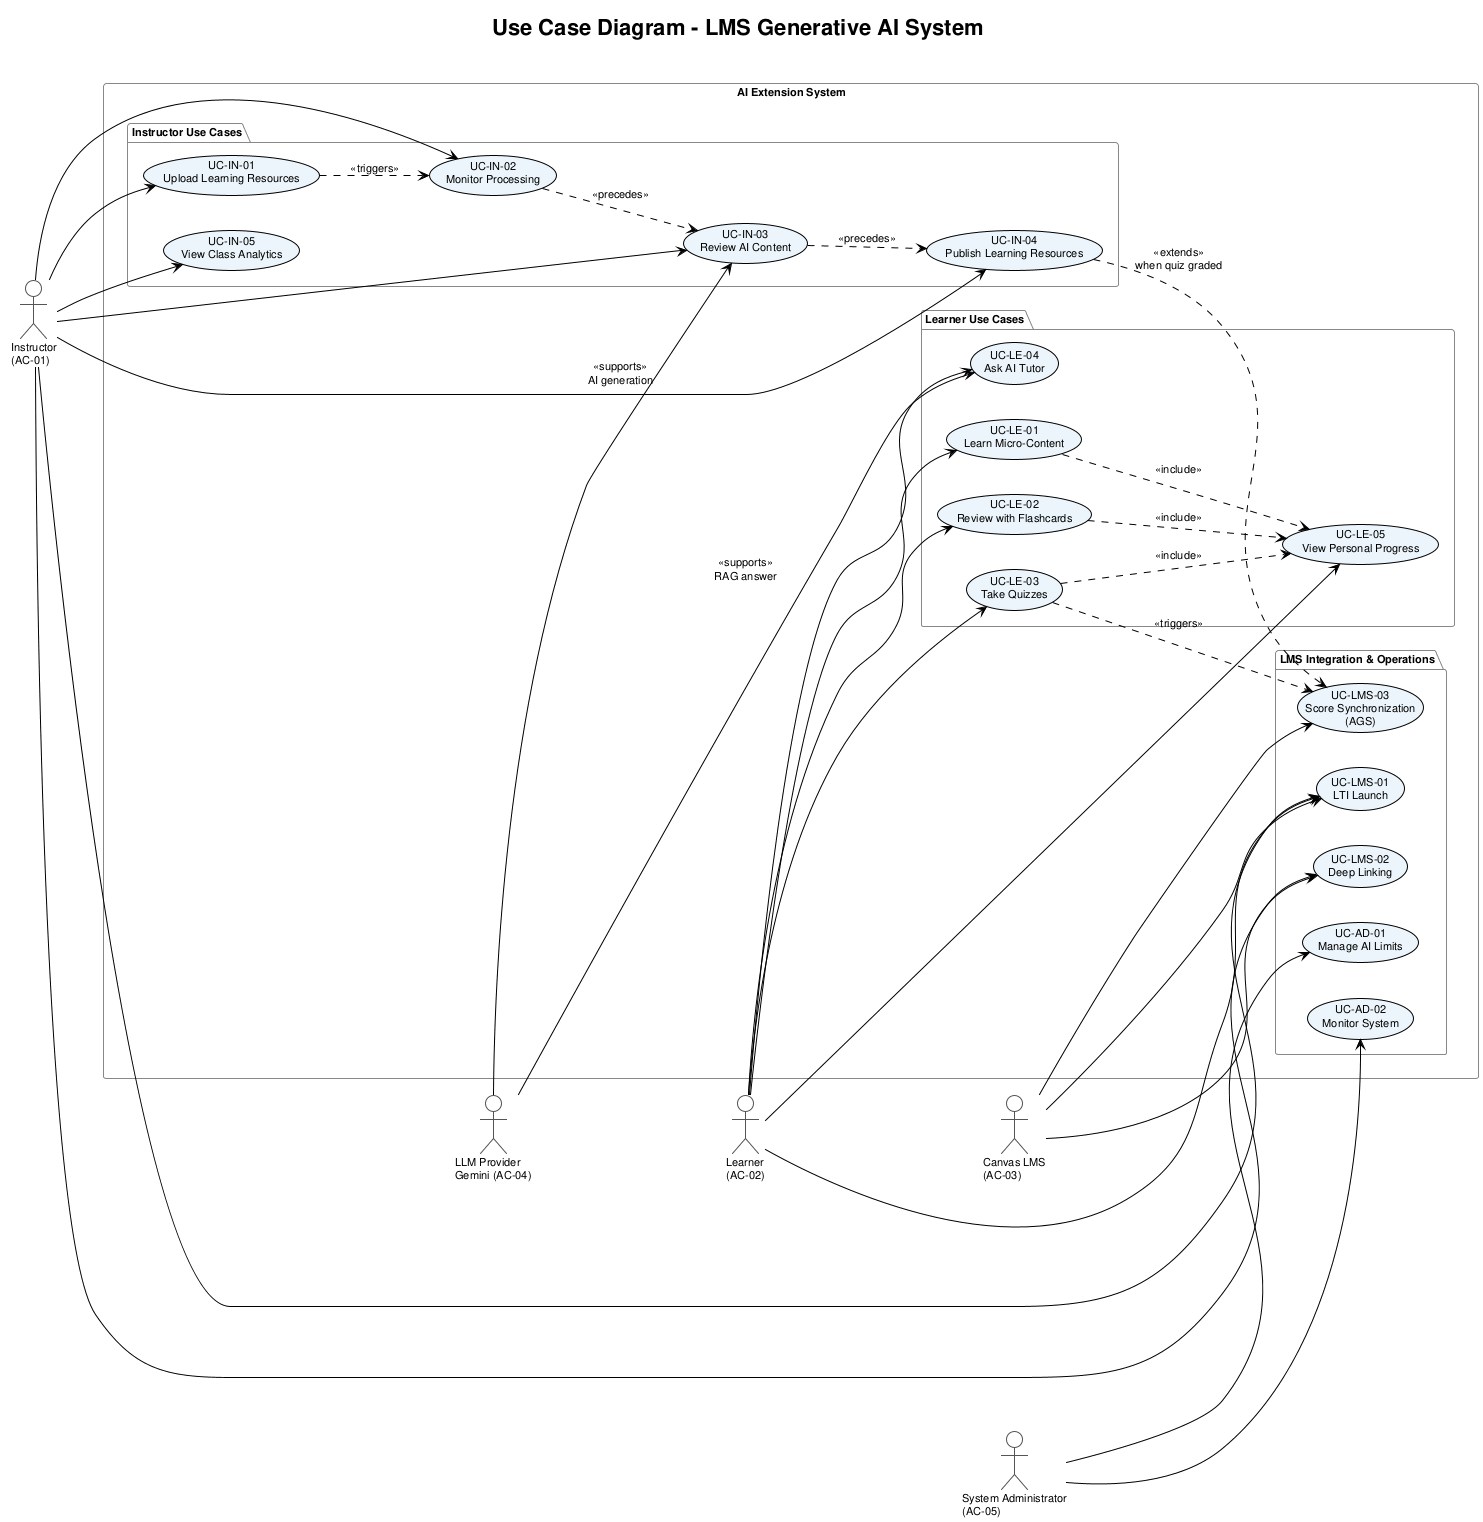
\includegraphics[width=\textwidth,height=0.85\textheight,keepaspectratio]{diagrams/usecase_diagram.png}
    \caption{Use case diagram of the LMS Generative AI system.}
    \label{fig:c2-usecase-diagram}
\end{figure}

Figure~\ref{fig:c2-usecase-diagram} shows the five actors of the system
(Instructor AC-01, Learner AC-02, Canvas LMS AC-03, LLM Provider AC-04,
and System Administrator AC-05) and the eighteen system-level use cases
they participate in. To make the responsibility of each actor easier to
inspect, the following subsections also provide actor-specific use case
views. These views do not introduce new use cases; they isolate each actor's
interactions from the system-level diagram. The remainder of this section
first lists every use case in tables with coverage columns grouped by actor
(Sections~\ref{subsec:use-case-tong-quan}--\ref{subsec:use-case-tich-hop-lms}),
then provides detailed specifications for the use cases that are
load-bearing for the thesis defense
(Section~\ref{subsec:main-use-case-specs}). Detailed specifications for
the remaining secondary use cases are gathered in
Appendix~\ref{appendix:use-case-reference}.

\subsection{System-level Use Case Overview}
\label{subsec:use-case-tong-quan}

At a high level, the proposed system operates as an AI extension tool for
Canvas LMS. Instructors and learners access it through LTI launch; the AI
system receives course context, processes learning resources, generates
content, supports learning, and synchronizes results when needed.
Table~\ref{tab:use-case-system-overview} summarizes the system-level grouping.

\begingroup
\small
\setlength{\tabcolsep}{3pt}
\begin{longtable}{|p{3.4cm}|p{4.2cm}|p{6.4cm}|}
\caption{System-level use case grouping}
\label{tab:use-case-system-overview}\\
\hline
\textbf{Group} & \textbf{Use cases} & \textbf{Main coverage} \\
\hline
\endfirsthead
\hline
\textbf{Group} & \textbf{Use cases} & \textbf{Main coverage} \\
\hline
\endhead
Access and LMS integration & UC-LMS-01--UC-LMS-03 & LTI launch, Deep Linking placement, and Canvas grade synchronization. \\
\hline
AI-assisted authoring & UC-IN-01--UC-IN-06 & Resource upload/lifecycle, syllabus and video ingestion, processing status, AI review, publishing, and class analytics. \\
\hline
Learner experience & UC-LE-01--UC-LE-06 & Micro-content/video learning, flashcards, quizzes, AI Tutor, semantic search, and personal progress. \\
\hline
Governance and operations & UC-AD-01--UC-AD-03 & AI quota, monitoring, incident visibility, and LMS tool configuration. \\
\hline
\end{longtable}
\endgroup

\subsection{Instructor Use Case Group}
\label{subsec:use-case-giang-vien}

Figure~\ref{fig:c2-usecase-instructor} isolates the instructor-facing
responsibilities: launching the tool from Canvas, preparing learning
resources, monitoring the AI pipeline, reviewing generated content,
publishing reviewed materials, managing resource lifecycle, and viewing
class-level analytics.

\begin{figure}[H]
    \centering
    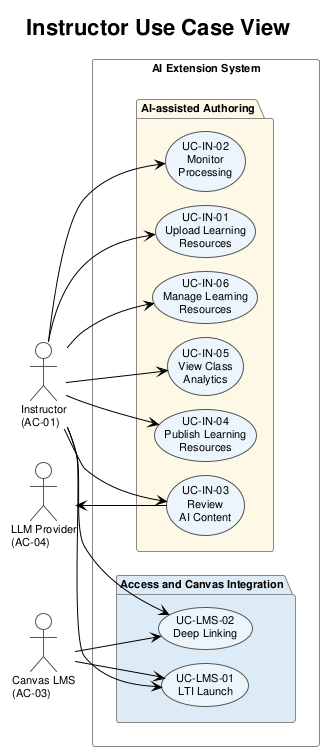
\includegraphics[width=\textwidth,height=0.55\textheight,keepaspectratio]{diagrams/usecase_instructor.png}
    \caption{Instructor use case view.}
    \label{fig:c2-usecase-instructor}
\end{figure}

\begingroup
\scriptsize
\setlength{\tabcolsep}{3pt}
\begin{longtable}{|p{1.8cm}|p{3.4cm}|p{4.0cm}|p{5.2cm}|}
\caption{Instructor use case group}
\label{tab:use-case-giang-vien}\\
\hline
\textbf{Code} & \textbf{Use case} & \textbf{Covered stories / requirements} & \textbf{Scope} \\
\hline
\endfirsthead
\hline
\textbf{Code} & \textbf{Use case} & \textbf{Covered stories / requirements} & \textbf{Scope} \\
\hline
\endhead
UC-IN-01 & Upload learning resources & US-IN-02, US-IN-03, US-IN-12; FR-LR-01--FR-LR-05, FR-SL-01 & Upload PDF, DOCX, PPTX, course syllabi, or lecture videos; start the asynchronous extraction, chunking, embedding, and generation pipeline. \\
\hline
UC-IN-02 & Monitor processing & US-IN-04; FR-AD-03 & View pipeline states such as queued, parsing, chunking, embedding, generating, completed, failed, and retrying. \\
\hline
UC-IN-03 & Review AI content & US-IN-05, US-IN-06, US-IN-07; FR-AI-01--FR-AI-04, FR-AI-06, FR-SL-03 & Preview, edit inline, add manual quiz questions, selectively regenerate, and approve / request changes / reject AI-generated content. \\
\hline
UC-IN-04 & Publish learning resources & US-IN-08; FR-AI-05, FR-SL-06 & Publish reviewed lessons, cards, flashcards, and quizzes to learners; unpublish when correction is needed. \\
\hline
UC-IN-05 & View class analytics & US-IN-09; FR-AD-01, FR-SL-05 & Track active learners, completion rate, average quiz score, weak Learning Outcomes, and content needing intervention. \\
\hline
UC-IN-06 & Manage learning resources & US-IN-11; FR-LR-07, FR-AD-05 & View, rename, delete, and rerun processing for documents/videos while preserving audit history and idempotent cleanup. \\
\hline
\end{longtable}
\endgroup

\subsection{Learner Use Case Group}
\label{subsec:use-case-hoc-vien}

Figure~\ref{fig:c2-usecase-learner} shows the learner-facing use cases.
Learners access the tool through Canvas, consume published micro-content,
review flashcards, take quizzes, search course content, ask the AI Tutor,
and inspect their own learning progress.

\begin{figure}[H]
    \centering
    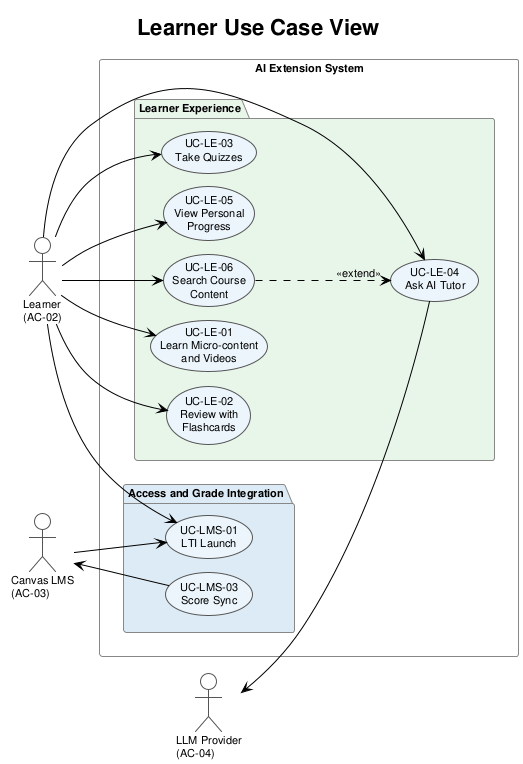
\includegraphics[width=\textwidth,height=0.55\textheight,keepaspectratio]{diagrams/usecase_learner.png}
    \caption{Learner use case view.}
    \label{fig:c2-usecase-learner}
\end{figure}

\begingroup
\scriptsize
\setlength{\tabcolsep}{3pt}
\begin{longtable}{|p{1.8cm}|p{3.4cm}|p{4.0cm}|p{5.2cm}|}
\caption{Learner use case group}
\label{tab:use-case-hoc-vien}\\
\hline
\textbf{Code} & \textbf{Use case} & \textbf{Covered stories / requirements} & \textbf{Scope} \\
\hline
\endfirsthead
\hline
\textbf{Code} & \textbf{Use case} & \textbf{Covered stories / requirements} & \textbf{Scope} \\
\hline
\endhead
UC-LE-01 & Learn micro-content and videos & US-LE-01, US-LE-02, US-LE-06, US-LE-09; FR-AI-05, FR-LR-02 & Read published summaries/cards, watch lecture video segments with timestamp cards, and resume from the last saved position. \\
\hline
UC-LE-02 & Review with flashcards & US-LE-03; FR-SL-02 & Flip flashcards, mark mastered / review again, and persist personal review state. \\
\hline
UC-LE-03 & Take quizzes & US-LE-04, US-IN-10; FR-SL-04, FR-SL-06 & Take quizzes, receive immediate feedback and explanations, and trigger grade synchronization when the activity is gradable. \\
\hline
UC-LE-04 & Ask AI Tutor & US-LE-07; FR-CHAT-01--FR-CHAT-05 & Ask natural-language questions and receive course-scoped, cited, retrieval-grounded answers. \\
\hline
UC-LE-05 & View personal progress & US-LE-08; FR-AD-02, FR-SL-05 & View completed sections, quiz score trends, and Learning Outcomes that need review. \\
\hline
UC-LE-06 & Search course content & US-LE-05; FR-LR-06 & Search published cards, chunks, and transcript segments in Vietnamese or English with source references. \\
\hline
\end{longtable}
\endgroup

\subsection{LMS Integration and Operations Use Case Group}
\label{subsec:use-case-tich-hop-lms}

The remaining actor-specific views clarify the supporting actors around the
AI extension. Canvas LMS provides identity, course context, deep-link
placement, and score synchronization
(Figure~\ref{fig:c2-usecase-canvas-lms}). The LLM Provider is not a
separate business user; it is a supporting external service invoked by AI
generation and AI Tutor interactions
(Figure~\ref{fig:c2-usecase-llm-provider}). The System Administrator manages
Canvas tool configuration, operational limits, and system health
(Figure~\ref{fig:c2-usecase-admin}).

\begin{figure}[H]
    \centering
    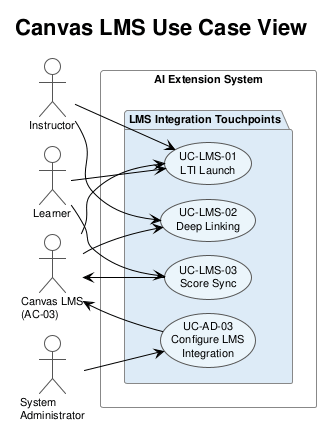
\includegraphics[width=0.92\textwidth,height=0.42\textheight,keepaspectratio]{diagrams/usecase_canvas_lms.png}
    \caption{Canvas LMS use case view.}
    \label{fig:c2-usecase-canvas-lms}
\end{figure}

\begin{figure}[H]
    \centering
    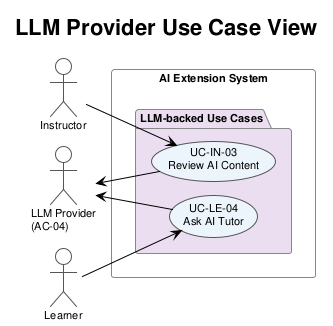
\includegraphics[width=0.92\textwidth,height=0.42\textheight,keepaspectratio]{diagrams/usecase_llm_provider.png}
    \caption{LLM Provider use case view.}
    \label{fig:c2-usecase-llm-provider}
\end{figure}

\begin{figure}[H]
    \centering
    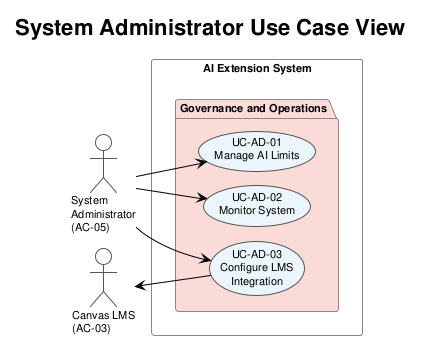
\includegraphics[width=0.92\textwidth,height=0.42\textheight,keepaspectratio]{diagrams/usecase_admin.png}
    \caption{System Administrator use case view.}
    \label{fig:c2-usecase-admin}
\end{figure}

\begingroup
\scriptsize
\setlength{\tabcolsep}{3pt}
\begin{longtable}{|p{1.8cm}|p{3.4cm}|p{4.0cm}|p{5.2cm}|}
\caption{LMS integration and operations use case group}
\label{tab:use-case-lms-van-hanh}\\
\hline
\textbf{Code} & \textbf{Use case} & \textbf{Covered stories / requirements} & \textbf{Scope} \\
\hline
\endfirsthead
\hline
\textbf{Code} & \textbf{Use case} & \textbf{Covered stories / requirements} & \textbf{Scope} \\
\hline
\endhead
UC-LMS-01 & LTI launch & US-IN-01, US-LE-01; security NFRs & Canvas authenticates the user and passes course, role, and resource context to the AI system. \\
\hline
UC-LMS-02 & Deep Linking & US-IN-08; LTI Advantage integration & The instructor selects content or an activity from the AI system and attaches it to the Canvas course. \\
\hline
UC-LMS-03 & Score synchronization & US-IN-10, US-LE-04; FR-SL-06 & The system sends quiz scores or completion status to Canvas Gradebook when the activity is graded. \\
\hline
UC-AD-01 & Manage AI limits & US-AD-02; FR-AD-04 & The administrator configures quota, LLM call limits, and cost alert thresholds. \\
\hline
UC-AD-02 & Monitor system & US-AD-03; FR-AD-03, FR-AD-05 & The administrator monitors logs, errors, latency, job queues, audit events, and AI usage cost. \\
\hline
UC-AD-03 & Configure LMS integration & US-AD-01; LTI/OIDC configuration & The administrator registers and validates Canvas Developer Key, deployment, redirect URLs, JWKS, Deep Linking, and AGS settings. \\
\hline
\end{longtable}
\endgroup

\subsection{Detailed Specifications of Main Use Cases}
\label{subsec:main-use-case-specs}

The seven main use cases below are specified in full because they
exercise the load-bearing architectural decisions of the thesis: LTI
integration, the document/AI pipeline, the human-in-the-loop review
gate, and the RAG-grounded learner experience. The remaining eleven
secondary use cases are specified with the same template in
Appendix~\ref{appendix:use-case-reference}.

\subsubsection*{UC-IN-01 -- Upload Learning Resources}

\begin{longtable}{|p{3.2cm}|p{10.3cm}|}
\hline
\textbf{Field} & \textbf{Specification} \\
\hline
\endhead
Primary actor & Instructor (AC-01) \\
\hline
Secondary actors & Canvas LMS (LTI launch context), AI Pipeline (triggered) \\
\hline
Preconditions & Instructor launched the tool from Canvas with role
    \texttt{Instructor}; an internal session exists; the target course
    is bound via \texttt{lms\_course\_ref}. \\
\hline
Main flow &
    1.\ Instructor selects PDF/DOCX/PPTX (or video) on the upload page.
    2.\ \texttt{web-bff} requests an upload session from \texttt{core-api}.
    3.\ \texttt{core-api} creates a \texttt{documents} row in status
    \texttt{UPLOADING} and returns a MinIO presigned URL.
    4.\ Browser uploads the file directly to MinIO.
    5.\ \texttt{web-bff} confirms the upload; \texttt{core-api} flips
    status to \texttt{QUEUED} and publishes
    \texttt{DocumentUploaded}/\texttt{VideoUploaded} on BullMQ. \\
\hline
Postconditions & A row exists in PostgreSQL, the file lives in MinIO,
    and the document/video pipeline (UC-IN-02) is triggered
    asynchronously. \\
\hline
Alternate flows &
    \emph{A1} - Invalid file type or size: \texttt{core-api} returns
    HTTP 422; status set to \texttt{ERROR}; instructor sees an inline
    error.
    \emph{A2} - Upload aborted by browser: the presigned URL expires;
    the row remains in \texttt{UPLOADING} and is garbage-collected by a
    scheduled job after 24h.
    \emph{A3} - Syllabus upload: the curriculum extractor creates a
    draft Course/Chapter/LO structure for instructor confirmation.
    \emph{A4} - Video upload: \texttt{VideoUploaded} starts transcript
    extraction and timestamp-based segment processing. \\
\hline
\end{longtable}

\subsubsection*{UC-IN-03 -- Review AI Content}

\begin{longtable}{|p{3.2cm}|p{10.3cm}|}
\hline
\textbf{Field} & \textbf{Specification} \\
\hline
\endhead
Primary actor & Instructor (AC-01) \\
\hline
Preconditions & At least one card or quiz item exists with status
    \texttt{GENERATED\_DRAFT} or \texttt{CHANGES\_REQUESTED} for a
    course owned by the instructor. \\
\hline
Main flow &
    1.\ Instructor opens \texttt{/manage/review}; \texttt{web-bff}
    fetches the review inbox grouped by lesson.
    2.\ Instructor opens a draft item; the system shows content plus
    citations (source chunks / video timestamps).
    3.\ Instructor edits inline; \texttt{core-api} persists the change
    and writes a \texttt{review\_audit\_logs} row.
    4.\ Instructor can add a manual quiz item or request selective
    regeneration for one card, section, or quiz set.
    5.\ Instructor chooses Approve, Request Changes, or Reject.
    6.\ \texttt{core-api} transitions the status accordingly and
    records the actor and diff in audit log. \\
\hline
Postconditions & Item is in \texttt{APPROVED} (eligible to publish),
    \texttt{CHANGES\_REQUESTED} (returned for regeneration), or
    \texttt{REVIEWING} (still in progress). Audit log captures all
    transitions. \\
\hline
Alternate flows &
    \emph{A1} - Instructor requests regeneration: a new
    \texttt{ContentGenerationRequested} event is enqueued; the old
    draft is archived.
    \emph{A2} - Bulk approve: instructor selects multiple items; the
    same flow runs in a single transaction. \\
\hline
\end{longtable}

\subsubsection*{UC-IN-04 -- Publish Learning Resources}

\begin{longtable}{|p{3.2cm}|p{10.3cm}|}
\hline
\textbf{Field} & \textbf{Specification} \\
\hline
\endhead
Primary actor & Instructor (AC-01) \\
\hline
Secondary actor & Canvas LMS (receives published resource via LTI Deep
    Linking when applicable). \\
\hline
Preconditions & All required cards/quiz items in the target Lesson are
    in status \texttt{APPROVED}. \\
\hline
Main flow &
    1.\ Instructor clicks Publish on a Lesson.
    2.\ \texttt{core-api} runs one PostgreSQL transaction:
    update status \texttt{APPROVED} $\to$ \texttt{PUBLISHED}, insert
    \texttt{outbox\_events} (\texttt{CardPublishedEvent} /
    \texttt{QuizPublishedEvent}).
    3.\ Outbox Poller dispatches a graph-sync job; worker MERGEs
    \texttt{Card}/\texttt{QuizItem} nodes into Neo4j with
    \texttt{EXPLAINS}/\texttt{ASSESSES} edges.
    4.\ Updates chunk Qdrant payload visibility to
    \texttt{all} so learners can retrieve them. \\
\hline
Postconditions & Learners can access the published content; the
    Knowledge Graph is eventually consistent with PostgreSQL. \\
\hline
Alternate flows &
    \emph{A1} - Not all items approved: Publish button is disabled
    with explanation.
    \emph{A2} - Unpublish: a reverse transition is recorded; visibility
    rolls back to \texttt{instructor} only. \\
\hline
\end{longtable}

\subsubsection*{UC-LE-01 -- Learn Micro-content and Videos}

\begin{longtable}{|p{3.2cm}|p{10.3cm}|}
\hline
\textbf{Field} & \textbf{Specification} \\
\hline
\endhead
Primary actor & Learner (AC-02) \\
\hline
Preconditions & Learner launched the tool from Canvas with role
    \texttt{Learner}; at least one Lesson or video segment in the course
    is \texttt{PUBLISHED}. \\
\hline
Main flow &
    1.\ Learner opens \texttt{/learn/lessons/\{id\}}; \texttt{web-bff}
    fetches published cards and optional video segment metadata.
    2.\ System displays cards in order; if the lesson has video
    timestamps, the player shows markers linked to the corresponding
    cards.
    3.\ \texttt{web-bff} reports view events to
    \texttt{learning\_events} for progress tracking.
    4.\ Learner can flip a card into flashcard mode and persist
    mastered / review-again state, or jump from a card to the matching
    video timestamp. \\
\hline
Postconditions & \texttt{learning\_events} and
    \texttt{flashcard\_reviews} updated; learner sees an updated
    progress indicator. \\
\hline
Alternate flows &
    \emph{A1} - Learner leaves mid-way: last position is autosaved;
    next launch resumes from there. \\
\hline
\end{longtable}

\subsubsection*{UC-LE-03 -- Take Quizzes}

\begin{longtable}{|p{3.2cm}|p{10.3cm}|}
\hline
\textbf{Field} & \textbf{Specification} \\
\hline
\endhead
Primary actor & Learner (AC-02) \\
\hline
Secondary actor & Canvas LMS (receives score via LTI AGS when the
    activity is gradable). \\
\hline
Preconditions & Quiz items in \texttt{PUBLISHED} status exist for the
    selected Lesson; a corresponding \texttt{lti\_line\_items} row
    exists if AGS passback is enabled. \\
\hline
Main flow &
    1.\ Learner opens \texttt{/learn/lessons/\{id\}/quiz}.
    2.\ Quiz items shown one by one; learner answers; system records
    \texttt{quiz\_attempts} with chosen answer.
    3.\ On submit, system grades and shows immediate feedback +
    explanation per item.
    4.\ If AGS-linked, \texttt{core-api} posts the score to
    \texttt{lti\_line\_items.lms\_line\_item\_url}; status flips
    \texttt{PENDING} $\to$ \texttt{POSTED}. \\
\hline
Postconditions & \texttt{quiz\_attempts} captures the score and
    grading; Canvas Gradebook reflects the score within $\leq 5$
    seconds. \\
\hline
Alternate flows &
    \emph{A1} - AGS POST fails: status \texttt{FAILED}; a retry job is
    scheduled.
    \emph{A2} - Quiz not gradable: skip AGS; status
    \texttt{NOT\_REQUIRED}. \\
\hline
\end{longtable}

\subsubsection*{UC-LE-04 -- Ask AI Tutor}

\begin{longtable}{|p{3.2cm}|p{10.3cm}|}
\hline
\textbf{Field} & \textbf{Specification} \\
\hline
\endhead
Primary actor & Learner (AC-02) \\
\hline
Secondary actor & LLM Provider (AC-04) -- supplies the streamed
    answer. \\
\hline
Preconditions & Course has at least one \texttt{PUBLISHED} content
    item; Qdrant has corresponding chunks with
    \texttt{visibility=all}. \\
\hline
Main flow &
    1.\ Learner types a question in the chat UI.
    2.\ \texttt{web-bff} requests a short-lived JWT from
    \texttt{core-api}; the JWT carries
    \texttt{allowed\_lo\_ids}/\texttt{allowed\_document\_ids}.
    3.\ \texttt{web-bff} opens SSE to \texttt{chat-service} with the
    JWT and question.
    4.\ \texttt{chat-service} runs hybrid retrieval on Qdrant (dense +
    sparse + RRF), graph-aware rerank on Neo4j, then calls the LLM
    streaming.
    5.\ Tokens stream back through SSE to the browser with inline
    citations. \\
\hline
Postconditions & \texttt{chat\_messages} stores question, answer,
    \texttt{chunks\_used}, and latency. \\
\hline
Alternate flows &
    \emph{A1} - Retrieval returns no relevant chunks: chat-service
    replies ``insufficient source material'' rather than fabricating
    an answer (refusal rule).
    \emph{A2} - LLM rate-limit/error: client receives an SSE error
    event and can retry. \\
\hline
\end{longtable}

\subsubsection*{UC-LMS-01 -- LTI Launch}

\begin{longtable}{|p{3.2cm}|p{10.3cm}|}
\hline
\textbf{Field} & \textbf{Specification} \\
\hline
\endhead
Primary actor & Canvas LMS (AC-03) -- initiates the launch on behalf
    of a Canvas user. \\
\hline
Secondary actors & Instructor or Learner (AC-01/AC-02) -- the human
    triggering the launch. \\
\hline
Preconditions & The system is registered in Canvas as an LTI 1.3 tool
    with a Developer Key; the user is enrolled in the course. \\
\hline
Main flow &
    1.\ User clicks the LTI activity in Canvas.
    2.\ Canvas calls \texttt{/lti/login} with
    \texttt{iss}, \texttt{client\_id}, \texttt{login\_hint}.
    3.\ \texttt{web-bff} stores state/nonce in Redis and redirects to
    Canvas \texttt{authorize\_redirect}.
    4.\ Canvas authenticates the user, POSTs \texttt{id\_token} back
    to \texttt{/lti/launch}.
    5.\ \texttt{web-bff} verifies the JWT (issuer, audience, signature
    via Canvas JWKS, exp, nonce, deployment\_id).
    6.\ Claims (\texttt{sub}, \texttt{context.id}, \texttt{roles},
    \texttt{custom.lesson\_id}) are extracted; \texttt{core-api}
    upserts \texttt{lms\_user\_mappings},
    \texttt{lms\_course\_ref}, \texttt{course\_memberships}.
    7.\ Server-side session is created in Redis; HttpOnly cookie set;
    user is redirected to the role-appropriate route. \\
\hline
Postconditions & The user has a valid internal session; user/course
    rows are kept in sync with the latest LTI claims; subsequent gRPC
    calls carry the BFF-signed internal JWT. \\
\hline
Alternate flows &
    \emph{A1} - JWT validation fails: HTTP 401; session not created;
    incident logged.
    \emph{A2} - State/nonce mismatch: launch rejected to prevent
    replay attacks. \\
\hline
\end{longtable}

\section{Functional Requirements by Module}
\label{sec:yeu-cau-chuc-nang-theo-module}

This section groups business requirements into major functional modules to
avoid duplication among business descriptions, user stories, and use cases.
Each requirement is assigned an \texttt{FR} code for traceability to design,
implementation, and testing.

\subsection{Learning Resource Management \& Processing Module}
\label{subsec:module-quan-ly-xu-ly-hoc-lieu}

This module receives documents/videos, processes input content, creates source
metadata, and provides semantic search for downstream AI modules.

\begin{longtable}{|p{2.4cm}|p{5.1cm}|p{6.9cm}|}
\caption{Functional requirements for the learning-resource management and processing module}
\label{tab:fr-hoc-lieu}\\
\hline
\textbf{Code} & \textbf{Requirement} & \textbf{Description / criteria} \\
\hline
\endfirsthead
\hline
\textbf{Code} & \textbf{Requirement} & \textbf{Description / criteria} \\
\hline
\endhead
FR-LR-01 & Document upload & Support PDF, DOCX, PPTX and validate format, size, and access rights by course. \\
\hline
FR-LR-02 & Video / audio upload & Support lecture videos, extract audio, create transcripts, and store timestamps for time-based learning. \\
\hline
FR-LR-03 & Content extraction & Parse text, headings, simple tables, slide text, and transcripts into normalized data. \\
\hline
FR-LR-04 & Chunking and metadata & Split content into chunks with \texttt{document\_id}, \texttt{chunk\_id}, page, heading path, timestamp, and processing status. \\
\hline
FR-LR-05 & Embedding and indexing & Create embeddings for chunks and store them in the vector database with metadata filters by course, document, and publish status. \\
\hline
FR-LR-06 & Semantic search & Allow instructors / learners to search in Vietnamese or English and return results with sources. \\
\hline
FR-LR-07 & Resource lifecycle management & Allow viewing, renaming, deleting, rerunning pipelines, and synchronizing state among storage, database, and vector index. \\
\hline
\end{longtable}

\subsection{AI Content Generation \& Control Module}
\label{subsec:module-kiem-soat-sinh-noi-dung-ai}

This module creates learning content using AI while keeping it under controls:
output schema, source citation, instructor review, and conditional publishing.

\begin{longtable}{|p{2.4cm}|p{5.1cm}|p{6.9cm}|}
\caption{Functional requirements for the AI content generation and control module}
\label{tab:fr-sinh-noi-dung-ai}\\
\hline
\textbf{Code} & \textbf{Requirement} & \textbf{Description / criteria} \\
\hline
\endfirsthead
\hline
\textbf{Code} & \textbf{Requirement} & \textbf{Description / criteria} \\
\hline
\endhead
FR-AI-01 & Generate lesson summaries & Create short summaries from chunks or sections, with traceable sources back to the original document. \\
\hline
FR-AI-02 & Generate key concept cards & Create cards by key concept, example, common misconception, and linked source chunk. \\
\hline
FR-AI-03 & Structured output & AI results must follow defined schemas; invalid data is rejected, retried, or moved to a needs-review state. \\
\hline
FR-AI-04 & Inline review & Instructors can edit content in place, mark accepted / needs changes, and preserve edit history. \\
\hline
FR-AI-05 & Controlled publishing & Only reviewed content can be published; learners only see the published version. \\
\hline
FR-AI-06 & Selective regeneration & Instructors can regenerate one card, one section, or one quiz set without rerunning the whole document pipeline. \\
\hline
\end{longtable}

\subsection{Intelligent Learning Module}
\label{subsec:module-hoc-tap-thong-minh}

This module focuses on quizzes and flashcards linked with curriculum structure,
Learning Outcomes, Bloom levels, and learner results.

\begin{longtable}{|p{2.4cm}|p{5.1cm}|p{6.9cm}|}
\caption{Functional requirements for the intelligent learning module}
\label{tab:fr-hoc-tap-thong-minh}\\
\hline
\textbf{Code} & \textbf{Requirement} & \textbf{Description / criteria} \\
\hline
\endfirsthead
\hline
\textbf{Code} & \textbf{Requirement} & \textbf{Description / criteria} \\
\hline
\endhead
FR-SL-01 & Learning Outcome management & Allow entering, extracting, or confirming LOs from the syllabus and mapping LOs with chapters / chunks. \\
\hline
FR-SL-02 & Flashcard generation & Generate two-sided flashcards from processed content and persist each learner's review state. \\
\hline
FR-SL-03 & Bloom-aware quiz generation & Generate questions with Bloom level, difficulty, answer, distractors, explanation, and source chunk. \\
\hline
FR-SL-04 & Quiz taking and feedback & Learners receive correct / incorrect feedback, explanations, and scores immediately after completing a quiz. \\
\hline
FR-SL-05 & Progress tracking by LO & The system aggregates scores and learning state by Learning Outcome to suggest review content. \\
\hline
FR-SL-06 & LMS score synchronization & When an activity is graded, the system sends scores to Canvas gradebook through the integration standard. \\
\hline
\end{longtable}

\subsection{AI Tutor Chatbot Module}
\label{subsec:module-ai-tutor-chatbot}

The chatbot module supports learners in asking questions according to course
context. Answers must be based on retrieval from published materials and
include sources for verification.

\begin{longtable}{|p{2.4cm}|p{5.1cm}|p{6.9cm}|}
\caption{Functional requirements for the AI Tutor Chatbot module}
\label{tab:fr-ai-tutor}\\
\hline
\textbf{Code} & \textbf{Requirement} & \textbf{Description / criteria} \\
\hline
\endfirsthead
\hline
\textbf{Code} & \textbf{Requirement} & \textbf{Description / criteria} \\
\hline
\endhead
FR-CHAT-01 & Course-scoped Q\&A & The chatbot only retrieves and answers within the course, role, and published content scope. \\
\hline
FR-CHAT-02 & RAG with citation & Each answer includes sources such as document, page, heading, card, or video timestamp when available. \\
\hline
FR-CHAT-03 & Refusal when sources are insufficient & If no suitable context is found, the chatbot reports insufficient information instead of inferring beyond the materials. \\
\hline
FR-CHAT-04 & Conversation history & Store questions, answers, used sources, latency, and user feedback for evaluation. \\
\hline
FR-CHAT-05 & Follow-up support & The chatbot keeps short-term conversation context but still retrieves sources again for subsequent questions. \\
\hline
\end{longtable}

\subsection{Administration \& Monitoring Module}
\label{subsec:module-quan-tri-theo-doi}

This module supports system administration, learning analytics, and AI pipeline
operation. It helps the system operate practically rather than remain a
content-generation prototype.

\begin{longtable}{|p{2.4cm}|p{5.1cm}|p{6.9cm}|}
\caption{Functional requirements for the administration and monitoring module}
\label{tab:fr-quan-tri-theo-doi}\\
\hline
\textbf{Code} & \textbf{Requirement} & \textbf{Description / criteria} \\
\hline
\endfirsthead
\hline
\textbf{Code} & \textbf{Requirement} & \textbf{Description / criteria} \\
\hline
\endhead
FR-AD-01 & Learning dashboard & Display class progress, quiz scores, completion rate, and weak Learning Outcomes. \\
\hline
FR-AD-02 & Personal dashboard & Learners view progress, learned content, quiz scores, and LOs needing review. \\
\hline
FR-AD-03 & Background job management & Monitor upload, parse, embedding, generation, retry, and pipeline-error jobs. \\
\hline
FR-AD-04 & AI quota management & Configure course / instructor limits, warn near quota, and block when thresholds are reached. \\
\hline
FR-AD-05 & Audit and change history & Record upload, review, publish, resource deletion, LLM calls, and score synchronization. \\
\hline
\end{longtable}

\section{Non-Functional Requirements}
\label{sec:yeu-cau-phi-chuc-nang}

Non-functional requirements describe the quality attributes the system must
satisfy during operation. These requirements directly affect architecture,
asynchronous pipeline deployment, storage selection, and security mechanisms.

\subsection{Performance and Scalability}
\label{subsec:hieu-nang-kha-nang-mo-rong}

\begin{itemize}
    \item Normal learning-interface APIs should respond in under 2 seconds
          under ordinary load.
    \item Heavy tasks such as document parsing, video processing, embedding,
          and LLM calls must run asynchronously through job queues.
    \item The system should support horizontal scaling of background workers as
          document or video volume increases.
    \item Vector search should support metadata filters by course, document,
          publish status, and access rights.
    \item Media files and raw documents should be stored in object storage to
          avoid bloating the relational database.
\end{itemize}

\subsection{Security and Privacy}
\label{subsec:bao-mat-quyen-rieng-tu}

\begin{itemize}
    \item Users accessing through Canvas must be authenticated using LTI 1.3 /
          OIDC; the system must not trust client data before token
          verification.
    \item Every access to documents, quizzes, chatbot, and analytics must check
          course context, role, and publish status.
    \item Learning materials, transcripts, questions, and learning history are
          sensitive data and must be access-limited by role.
    \item LLM Provider, storage, and LMS API keys must be stored in environment
          variables or a secret manager, not hard-coded in source code.
    \item Operational logs must not record secrets such as access tokens, API
          keys, or complete learner inputs unless necessary.
\end{itemize}

\subsection{Reliability and Maintainability}
\label{subsec:do-tin-cay-kha-nang-bao-tri}

\begin{itemize}
    \item Processing pipelines must have clear states: pending, processing,
          completed, failed, and retrying.
    \item Failed jobs need error reasons, retry counts, and controlled rerun
          capability.
    \item Modules interacting with LMS, LLM Provider, vector database, and
          object storage should be encapsulated behind adapters for easier
          replacement.
    \item AI-generated content must be stored with \texttt{prompt\_version},
          \texttt{model\_name}, \texttt{source\_chunk\_id}, and generation
          time for traceability.
    \item The system needs tests for important flows: LTI launch, upload,
          generation, review, publish, quiz submission, and chatbot retrieval.
\end{itemize}

\subsection{User Experience}
\label{subsec:trai-nghiem-nguoi-dung}

\begin{itemize}
    \item Instructors should clearly see processing status, errors, and next
          actions instead of guessing where the pipeline is.
    \item The review interface should support quick editing, section-level
          preview, and clear distinction among draft / reviewed / published
          content.
    \item Learners should access learning content inside Canvas without
          logging in again or understanding the AI system's technical details.
    \item Errors from LLM, upload, or retrieval should be user-friendly and
          should not expose stack traces to end users.
    \item The learning interface should be responsive for laptops and mobile
          devices, especially cards, flashcards, quizzes, and chatbot.
\end{itemize}

\section{AI-specific Requirements \& Monitoring}
\label{sec:yeu-cau-ai-giam-sat}

Unlike a traditional web system, an AI system has outputs that are not fully
deterministic and depend on retrieved data, prompts, models, and generation
configuration. Therefore, in addition to functional and non-functional
requirements, the system needs separate requirements for AI quality evaluation
and operational monitoring.

\subsection{AI System Evaluability}
\label{subsec:kha-nang-danh-gia-he-thong-ai}

\begin{itemize}
    \item The system must store evaluation data including prompts, model,
          retrieved context, answers, citations, and user feedback.
    \item Retrieval quality should be measured by metrics such as Recall@K,
          Precision@K, MRR, or nDCG on a test question set with source labels.
    \item Quiz content must be validated for schema, number of options, unique
          correct answer, explanation, Bloom level, and source chunk.
    \item Chatbot quality should be evaluated by source grounding, refusal to
          fabricate without context, usefulness, and answer clarity.
    \item The system should support comparison across prompt versions, models,
          chunking strategies, or embedding models to select suitable
          configurations.
\end{itemize}

\subsection{Observability and Monitoring}
\label{subsec:observability-monitoring}

\begin{itemize}
    \item The system must record structured logs for upload, parse, chunk,
          embedding, retrieval, generation, review, publish, and quiz
          submission.
    \item The operations dashboard should track active jobs, failed jobs,
          average processing time, LLM latency, token usage, and estimated
          cost.
    \item Each request to the LLM Provider should have a correlation id for
          tracing from UI, backend, and workers to provider logs if available.
    \item The system should alert when error rate, latency, queue length, or
          cost exceeds configured thresholds.
    \item Rate limiting, circuit breaking, or generation pause mechanisms are
          needed when providers fail repeatedly or cost exceeds quota.
\end{itemize}
